\documentclass[aspectratio=169]{beamer}

\usetheme{uniamntf}
% \usetheme[fai]{uniamntf} % fai-color

\title[small title]{The full Title}
\subtitle{subtitle}

\author{John Doe}
\institute[TP III]{Chair for theoretical Physics III}

\date[01.05.2024]{$1^{\text{st}}$ of Mai 2024}


\begin{document}

{
    % can be adapted to e.g. fai or mntf background
    \usebackgroundtemplate{
        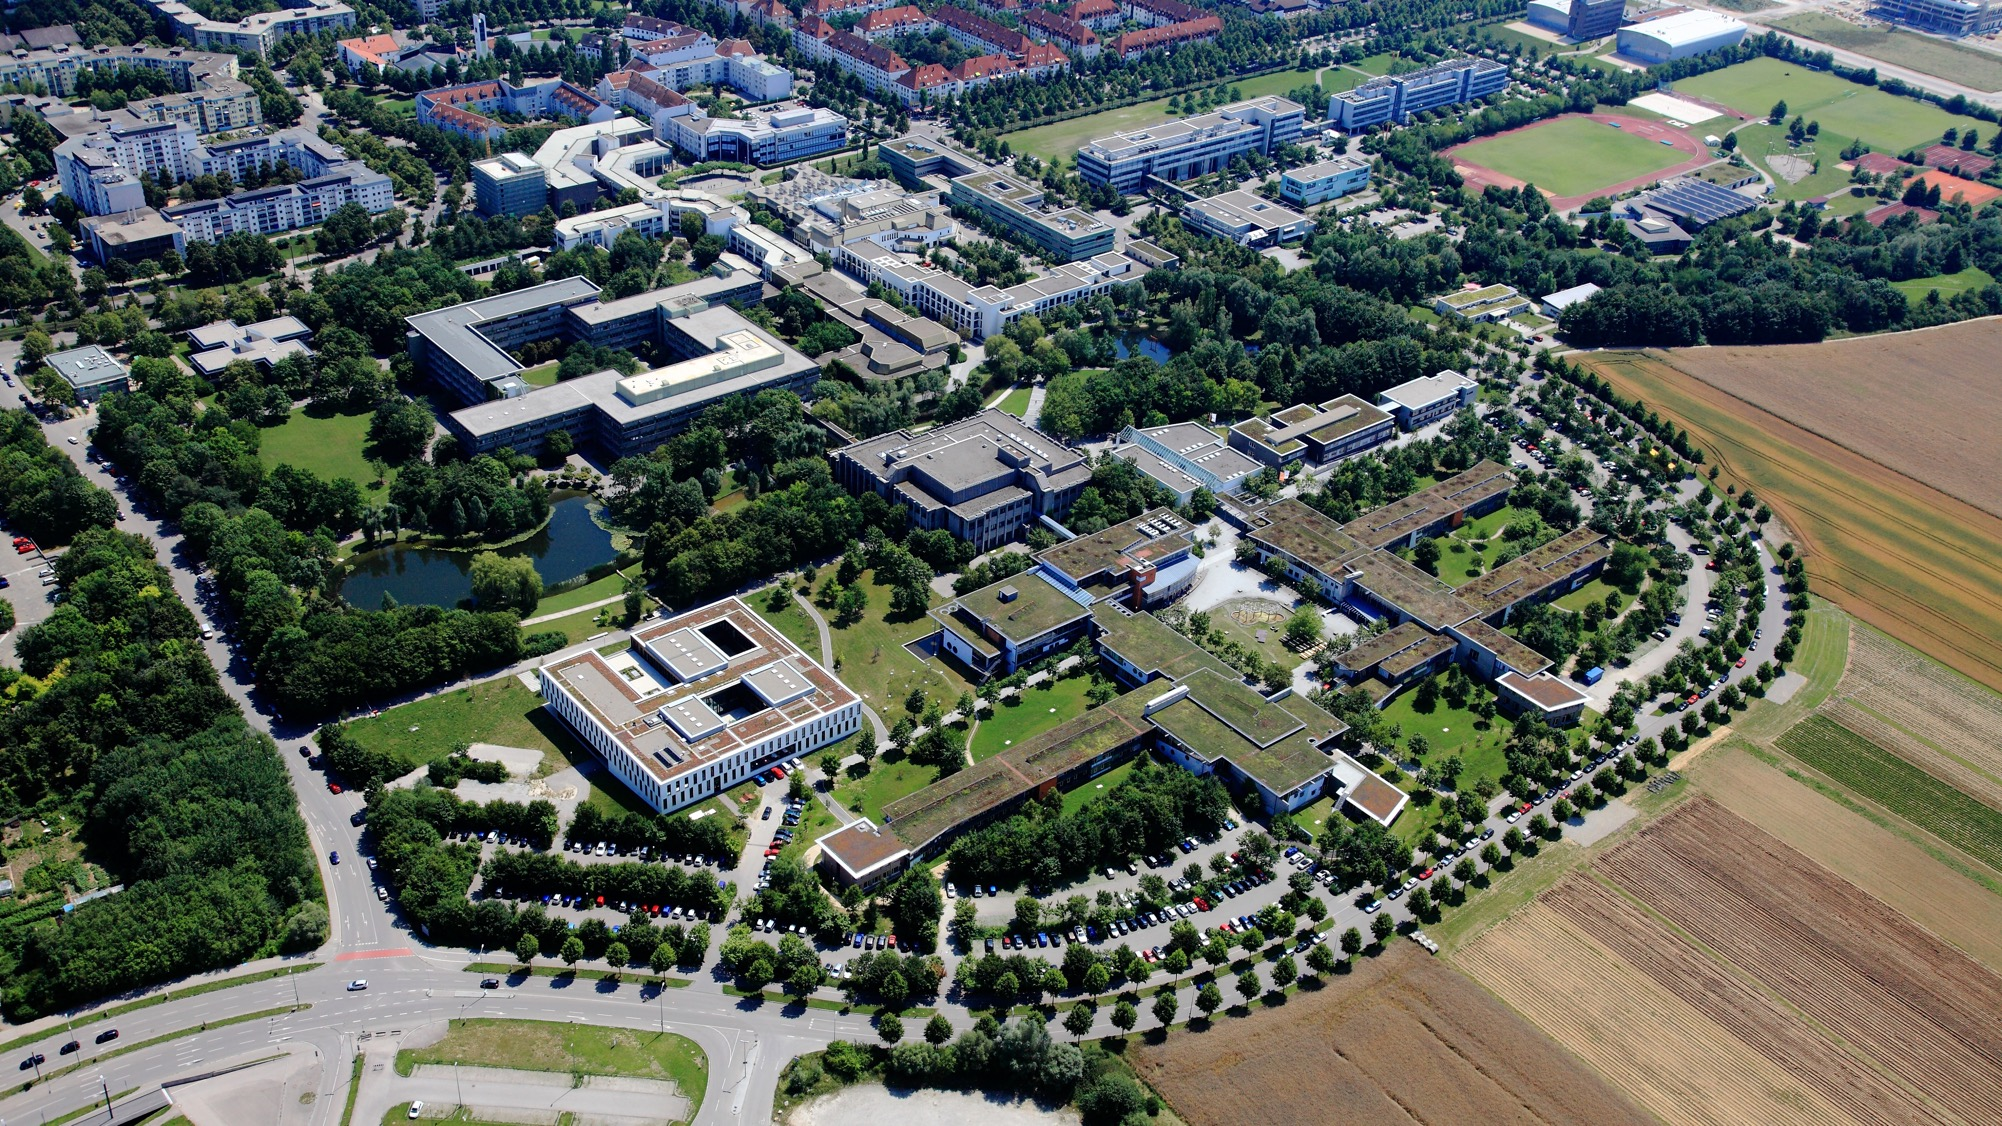
\includegraphics[width=\paperwidth,height=\paperheight]{slide-background-images/background-title-slide.png}
    }
    \begin{frame}[t,plain]
        \maketitle
    \end{frame}
}

\begin{frame}
    \frametitle{Outline}

    \tableofcontents

\end{frame}

\section{Testsection 1}

\begin{frame}
    \frametitle{Random Text}

    Hello\pause
    
    This is Text
\end{frame}

\begin{frame}
    \frametitle{Blocks}

    \begin{block}{Block}
        Sample text
    \end{block}

    \begin{exampleblock}{Example}
        Sample text
    \end{exampleblock}

    \begin{alertblock}{Conclusion}
        Sample text
    \end{alertblock}
\end{frame}

\section{Testsection 2}

\begin{frame}{Title-Here}
    \begin{columns}
        \column{0.4\textwidth}
            This is a text in first column.
            $$E=mc^2$$
            \begin{itemize}
                \item First item
                \item Second item
                \begin{itemize}
                    \item asdasd
                    \item asdasd
                    \begin{itemize}
                        \item asdasdasda
                        \item asdasdasd
                    \end{itemize}
                \end{itemize}
            \end{itemize}
        
        \column{0.4\textwidth}
            This text will be in the second column
            and on a second thoughts, this is a nice looking
            layout in some cases.
    \end{columns}
\end{frame}

\section{Testsection 3}
\subsection{sub-1}
\begin{frame}{ASD 1}
\end{frame}

\subsection{sub-2}
\begin{frame}{ASD 2}
\end{frame}


\end{document}